\newpage
\section{Extended State of the Art}\label{sec:eSOTA}

\begin{displayquote}
\textit{\textbf{\Huge{``}}}
\textit{\large{
Kubernetes has massive potential for handling IoT workloads on the edge by providing a common control plane across hybrid cloud and edge environments to simplify management and operations\cite{ioFogMainBlog:online}.
}}
\textit{\textbf{\Huge{''}}}
\\[1pt]
\raggedleft{{\rm --- Mike Milinkovich, CEO of Eclipse Foundation}}
\end{displayquote}

\comment{
https://www.iaria.org/conferences2016/filesICSNC16/Softnet2016_Tutorial_Fog-MEC-Cloudlets-E.Borcoci-v1.1.pdf

this paper has it nailed down with terms https://arxiv.org/pdf/1812.00591.pdf 
}

\subsection{Terms and Definitions} \label{sec:definitions}
The IoT and edge landscape is hard to understand, especially because terms are loosely and inconsistently defined. Similar is true for the cloud but it uses less diverse technologies and is thus less confusing. This section will explain the network topology, key terms and their concepts as the foundation for the following report.\\
\vspace{0.5mm} \ \\
\textbf{\textit{Network Topology}}\\
\Cref{fig:networkTopology3Layer} shows the network topology used in this report. 
% The focus will be on the management and security of the device edge as well as its interaction with the IoT devices themselves. 
\begin{figure}[H]
    \centering
    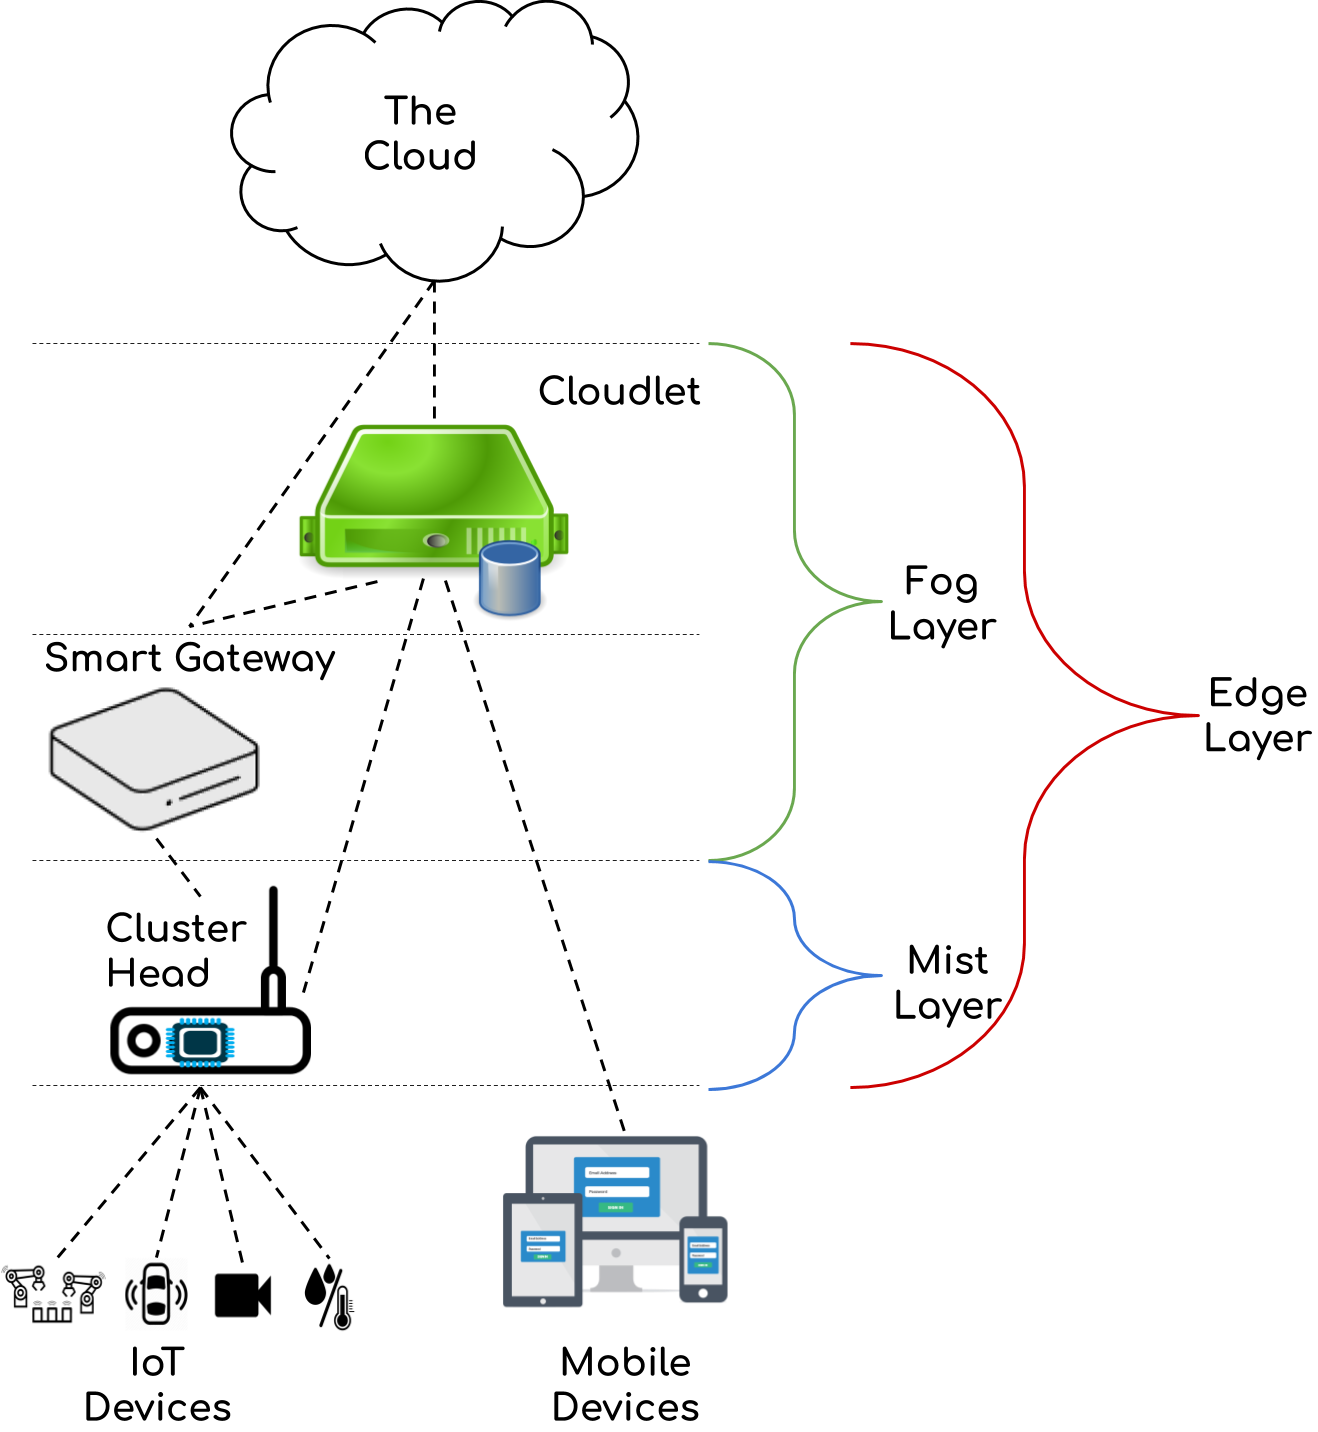
\includegraphics[scale=0.2]{figures/network-topology-3-layer.png}
    \caption{Three tier layer network topology, similar to \cite{nsa2017NextWaveIoTDef}}
    \label{fig:networkTopology3Layer}
\end{figure}

The cloud is well defined and understood. It describes the readily available computing resources over the Internet not managed by the user. The other layers and devices are not so well understood and defined separately.
\textbf{\textit{Constrained Device}}\\
Constraint devices are an elementary part of the IoT making up the "things"\cite{contstraintDevicesTerminology}.
They can have three main purposes. Either sensing or actuating (or both), where sensing is the 
passive action of measuring the environment (e.g. a motion detector) and actuating is the active action of influencing the environment (e.g. control of pressure in test tube). Or, finally, they can be smart objects enhancing the interaction between other smart objects and people.
They are usually defined by their limitation, mainly, small computing power (CPU, RAM, storage etc.) and limited power supply and operate in constrained network using protocols like BLE and ZigBee. \\[5mm]
\textbf{\textit{Smart/mobile devices}}\\
Smart devices are not clearly defined in the academic literature. I will use the definition given by \citeauthor{poslad2011smartDevices}\cite{poslad2011smartDevices}, to clearly divide them from constrained devices which this thesis will be concerned with. They are traditional computing devices and "tend to be multi purpose ICT devices"\cite{poslad2011smartDevices}, examples are mobile phones (smart phones) or tablets. They connect to the rest of the infrastructure directly but are free to move between networks. They also often rely on battery power and, importantly, are mainly end user devices. This has important privacy implication, a major factor for edge computing.\\[5mm]
\textbf{\textit{IoT Cluster Head}}\\
IoT Cluster Heads are defined by their very limited processing power. They are used to combine multiple sensors or actuators, but do not perform powerful operations. The line between IoT Cluster Heads and IoT Gateways is constantly moving as devices get more powerful and software more efficient. In this paper, IoT Cluster Heads are defined as devices which are used to read and control IoT devices but are not powerful enough to run containers or Kubernetes.
\textbf{\textit{IoT Gateway}}\\
IoT gateways are the connection between constrained devices and the cloud. I will use the term IoT gateway and not only gateway to stress its relation with IoT. They are usually connected to a network, either local or the the Internet. They facilitate inter-network and intra-network communications and because smart devices and especially constrained devices often communicate via wireless and non-Internet protocols, IoT gateways often translate protocols "between wireless sensor networks [...] and traditional communication networks"\cite{zhu2010iotGatewayDefinition}.
In recent years IoT Gateways have become a major field of interest and new research. As these devices got more powerful, developers started using them for pre-processing and data gathering locally at the edge.
IoT gateways can take a wide variety of forms. They can be simple L2/L3 routers or more powerful devices. Importantly, they are situated at the edge of a network.\\[5mm]
\textbf{\textit{Edge Layer}}\\
The edge layer is a term used to describe all resources sitting at the edge of the network. They do not interact with their environment directly only through IoT or mobile devices. This line started to fade, when mobile devices where used to control IoT devices directly. In this research I will stick to definition that edge layer devices are no user facing devices.\\[5mm]
\textbf{\textit{Fog Layer}}\\
The fog layer and consequently fog computing is a term used to describe the logical extension of traditionally cloud resources to the edge. These devices are still connected to the overall system and are an active part in the data processing pipeline. Fog computing enables repeatable structure on the edge for better and more scalable performance.
\textbf{\textit{Mist Layer}}\\
The mist layer is not logically connected to the cloud and both are not part of the same system and function independently of each other. It can be that the cloud can indirectly control the mist layer through the fog devices but importantly the mist layer does not do tasks which were traditional done in the cloud. \\[5mm]
\textbf{\textit{Edge cluster}}\\
Edge clusters are two or more edge devices working together where one device needs to be powerful enough to run a full control plane of the cluster technology. With emerging technologies like tiny builds of a full Kubernetes cluster, e.g. K3s from Rancher Labs\cite{k3sLight14:online}, this is becoming increasingly easier and more popular.
\footnote{Rancher provides a 40MB Kubernetes binary and claims that 500MB of RAM is sufficient 
it stable.}.\\
\textbf{\textit{Edge node}}\\
Edge nodes are defined as nodes "that act as an end user portal for communication with other
nodes in cluster computing"\cite{Whatised17:edgeNodeDef}. The other nodes can either be edge nodes as well or cloud nodes. Importantly, edge nodes do not need to be able to run their own control plane.
\subsection{Existing Solutions} \label{sec:existingSolutions}

Traditionally, edge devices were isolated cluster heads mainly forwarding traffic from their slaves to the cloud. Today, they are an integral part of the data flow pre-processing data and executing part of the business logic. But, there are still no coherent architectural as well as technological standards. In this section we will compare widely adopted and developed solutions in the industry to detect similarities and differences. The solutions also differ in age and 

% https://scholar.google.com/scholar?cluster=13680069378267225814&hl=de&as_sdt=0,5
% https://www.pac-online.com/sites/pac-online.com/files/upload_path/PDFs/Thema_des_Monats_Juni_2017_IoT_Plattformen.pdf
% https://blog.bosch-si.com/bosch-iot-suite/lessons-learned-using-kubernetes-in-iot-deployments/

\subsubsection{Bosch IoT Gateway Solutions}
\comment{https://www.bosch-iot-suite.com/service/gateway-software/}
The Bosch IoT Gateway Software\cite{BoschIoT13:online} is the "oldest" software analyzed. It is based on the OSGi technology\cite{osgiDefintion25:online}, which is an aliance driven project from the Open Services Gateway initiative (OSGi). It defines a set of specifications (with reference implemetation and tests) for a dynamic modular system based on so called bundles, third party software, running on the Java Virtual Machine (JVM)\footnote{This means it is possible to use other languages apart from Java which can run in a JVM, e.g. Kotlin.}. It is important to note that Bosch also supplies a cloud part which is based on Kubernetes.\\
The OSGi framework consists of a layered model shown in \cref{fig:osgiLayerModel}. 
\begin{figure}[h!]
    \centering
    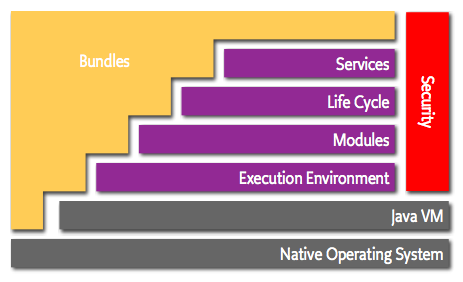
\includegraphics[scale=0.8]{figures/layering-osgi.png}
    \caption{From the official OSGI documentation\cite{osgiFrameworkArchitec22:online}.}
    \label{fig:osgiLayerModel}
\end{figure}
The Service layer interconnects the bundles making it possible for them to communicate via plain old java objects (POJO).The Life-Cycle layer handles the the state of the application (start, stop, update and uninstall). The Modules layer defines how an application can import and export code and the Execution Environemnt defines which methods and classes are available in a specific environemnt. Finally, the Security layer encompasses all other layers and handles for example code authentication, the digital signing of jar files, file access restrictions, certificates and more.\\
To the authors best knowledge there are currently five frameworks implementing the OSGi model besides the Bosch IoT Gateway Software\cite{BoschIoT13:online}. In a blog entry from 2015 Bosch compares the OSGi technology to other gateway solutions and says it "is the only one with clearly defined specs and an open specification process behind them"\cite{boschBlogOSGi69:online}. Boschs solution is proprietary and tailor made for edge-computing devices with IIoT in mind\cite{OSGiforIoTBlog27:online}. It runs on Linux, Windows, mac OS, Android, and VxWorks and according to Bosch more than 40 different gateway devices\cite{BoschIoT13:online}. The software is stable at major version 9 and still under heavy development. It is presented as exemplary software by the OSGi Alliance for IoT Gateways \cite{exampleIoTGateweOSGi:online} and thus used in this report. \Cref{fig:boschIoTGatewaySetup} shows where Boschs IoT solution is situated in the IoT environment. Bosch provides the OSGi framework implementation for the gateways and additional features for the cloud to ease the management of the gateways and store the accumulated data.
\begin{figure}[h!]
    \centering
    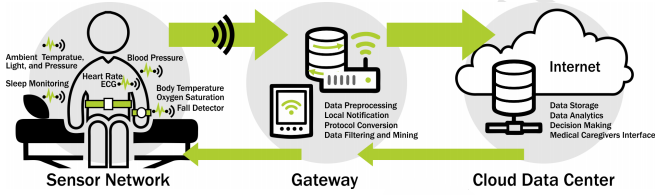
\includegraphics[scale=0.8]{figures/iotSetup.png}
    \caption{From the official Bosch documentation \cite{BoschIoT13:online}.}
    \label{fig:boschIoTGatewaySetup}
\end{figure}
Moreover, it supports a wide variety of communication protocls, BLE, ZigBee and MQTT, just to name a few. The main restriction is the JVM support for a protocol.  

\subsubsection{ioFog}
ioFog is one of the older projects in this report, with the first official release in 2016\cite{ioFogMainBlog:online}. Similarly to the OSGi framework it provides a runtime environment for applications, mainly intended for microservices. In addition, it includes a message bus, dynamic configuration of the microservices, and remote debugging\cite{ioFogMainBlog:online}. It runs on (almost) all Linux distributions and only requires Docker to be installed. In their official system requirements they only recommed using a Raspberry Pi as a worker node and not to run the Controller and Connector infrastructure \cite{ioFOgQuickStart:online}.
\Cref{fig:ioFogComponent} shows the fog computing layers in more detail.
\begin{figure}[h!]
    \centering
    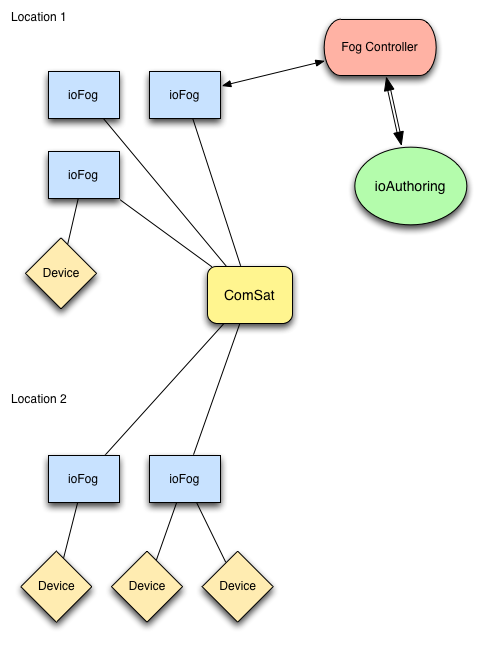
\includegraphics[scale=0.4]{figures/ioFog-Component_Diagram.png}
    \caption{hallo}
    \label{fig:ioFogComponent}
\end{figure}\\
The ioAuthoring application and the ioFog instances provide orchestration and management of the microservices. They are the main interaction points between the administrator and the system.
The fog computing software agent, called "ioFog", runs on various operating systems and provides a universal runtime for the IoT microservices. It includes a Software Development Kits (SDKs) in multiple programming languages to provide developers with the convenience of programming against standardized objects. The communication between different ioFog instances is facilitated through an internetworking utility that runs on popular Linux distributions, called "ComSat". Finally, for testing a tool for mimicking the fog computing runtime is included as well.\\
In a recent blog post from Mike Milinkovich, the Executive Director of the Eclipse Foundation Inc., he announced the initial availability of ioFog features that make any Kubernetes distribution edge-aware. He continuous saying that "these native Kubernetes enhancements are in the process of being contributed to the Eclipse ioFog open source project.", so not all features are available in the stable release as of the time of writing. But essentially, the ioFog Kubernetes APIs would provide standardized way of communication between the Kubernetes API Server and the ioFog instance.

\subsubsection{Docker Edge Solution}
Docker is commonly known for its containerization software and is often confused with the containers themselves (like google for search). The core container runtime, containerd, was donated by Docker to the Cloud Native Computing Foundry (CNCF) in 2017\cite{containerDonationDocker79:online} which manages and develops it now. Now, the company Docker focuses on providing an ecosystem around containers making them easy to deploy, secure and replicate. Recently, Docker announced a new partnerships with ARM and  a new strategy for edge devices.\\
\Cref{fig:dockerEdge} shows the Docker Edge Solution in context. 
\begin{figure}[h!]
    \centering
    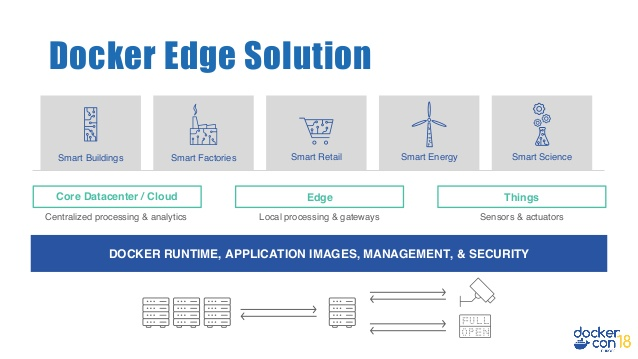
\includegraphics[scale=0.65]{figures/docker-edge-solution.jpg}
    \caption{Docker Edge solution .}
    \label{fig:dockerEdge}
\end{figure}
The solution consists of a few different products from its enterprise solution focusing on security, scalability/deployability and easy of use. The components are the same, but the edge focus is on fault tolerance and platform support, hence the new partnership with ARM. A core component of the suit is the docker registry, which can be mirrored/replicated on many difference servers for scaleability and fault tolerance. The edge registry can function without constant communication with the rest of the swarm. In case of no connection, the registry will only pull images which it already posses. As edge devices often have limitted disk space, docker only synchronizes promoted images on these nodes. Similarly to tags in git, promoted images are signed images that are explicitly marked as production ready. \cref{fig:dockerRegistryForIoT} shows registry management in the cloud (on the left) vs. on the edge (on the right).
\begin{figure}[h!]
    \centering
    \noindent\makebox[\textwidth]{
    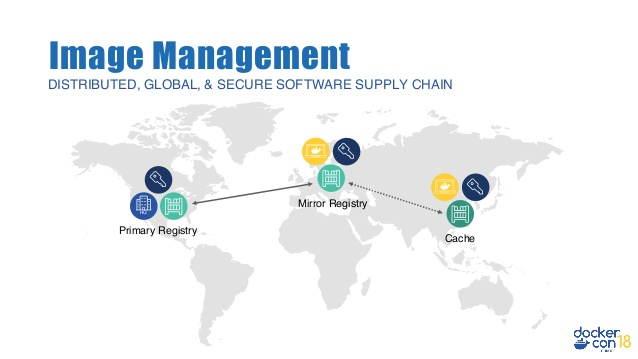
\includegraphics[width=(\textwidth+4cm)/2]{figures/docker-edge-computing-with-docker-enterprise.jpg}
    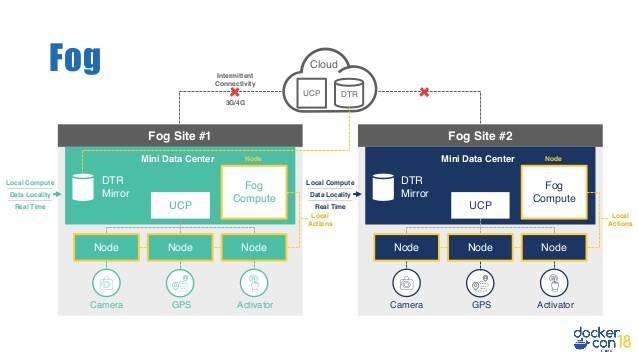
\includegraphics[width=(\textwidth+4cm)/2]{figures/docker-edge-registry-mirror.jpg}}
    \caption{The Docker registry in the cloud (left) vs. on the edge (right).}
    \label{fig:dockerRegistryForIoT}
\end{figure}
Whereas the cloud registry is build high availability (HA/LB) of the nodes in the swarm with fault tolerance against other nodes being unavailable, the edge registry is designed to have fault tolerance on it's own Internet access. In case of no connection it works as a standalone component, but synchronizes itself when it has a connection.\\
Importantly, the Docker Edge Solution is not a standalone solution, but integrates into the Docker ecosystem enabling remote management.

\subsubsection{K3s}
K3s is a "lightweight" kubernetes\footnote{Kubernetes is also known as k8s, hence the name k3s.} fork developed by Rancher\cite{rancherMainPage:online}. Similarly to Kubernetes and containerd, k3s is an open source project under the official management of the CNCF. It is also part of the Kubernetes IoT Edge working group explicitly aiming at bringing kubernetes related technologies to the edge. K3s is also a Certified Kubernetes distribution, meaning it confirms with the Kubernetes API standards. One of its big selling points is the good support for ARM64 and ARMv7 (targeting the Raspberry Pi and other smaller/less powerful single board computers). The traditional Kubernetes development is focused around the x86\_64 architecture, with limitted, and often untested, support for ARM, especially ARMv7. The co-founders of Rancher and developers behind k3s actually state in a webinar that half their development effort went into ensuring that all features they wanted work seamlessly on ARM\cite{k3sTalk:online}.\\
On their k3s product page \url{https://k3s.io/} Rancher describes the fork as follows:
\begin{displayquote}
Easy to install. A binary of less than 40 MB. Only 512 MB of RAM required to run.
\end{displayquote}
So k3s is not only significantly smaller than the full fledged Kubernetes install, but also requires significantly less resources at run time. It achieves this by mainly slimming down Kubernetes only including what they deem important for the edge. Because of the huge popularity of Kubernetes, it needs to support legacy code, drivers etc. K3s is free to break compatibility with older versions and the developers can instead focus on slimming down the code base much as possible. The lead developer, Darren Shepherd, said:
\begin{displayquote}
\textit{"We took Kubernetes and ripped out every single feature we didn't want.\cite{k3sTalk:online}"}
\\[1pt]
\raggedleft{{\rm --- Darren Shepherd}}
\end{displayquote}
K3s also integrates all process required by Kubernete, the Kubernetes master, Kubelet and containerd under one system process which requires less memory in total. \\
Another important aspect of k3s is its purpose to run on single as well as multi-node clusters. This is in stark contrast to Kubernetes, which is intended to run inside a cluster and it's fault tolerance model is build around on a multi-node cluster structure. Running a single node cluster is possible, but requires the tainting of the master node and is describe as "cheap and easy, but is not production grade" in the official documentation\cite{singleNodeKubernetesNotProductionDocumenhtation:online}.

\subsubsection{Kubeedge}
Kubeedge is another project inside the Kubernetes IoT Edge working group and thus build with Kubernetes in mind. It is a relatively young project to extend native containerized application orchestration and device management to the Edge. It is based on two parts, the cloud and the edge and (mainly) developed by Huawei, which at the time of writing could be reason for future complications because of recent US sanctions against the company.\\
The kubeedge system is shown in \cref{fig:kubeedgeStruct}.
\begin{figure}[h!]
    \centering
    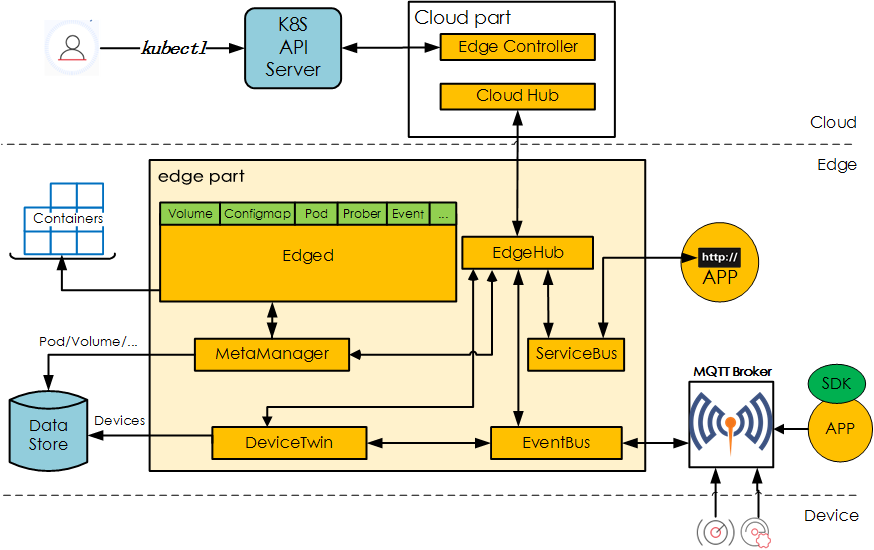
\includegraphics[width=(\textwidth+4cm)/2]{figures/kubeedge_arch.png}
    \caption{The Kubeedge system design.}
    \label{fig:kubeedgeStruct}
\end{figure}
The cloud part is built upon Kubernetes and provides support for application deployment, metadata synchronization and networking all through the Kubernetes API Server. The cloud and edge part communicate via web sockets. This means by design a good connection to the server is expected and the intend of the authors is to enable Fog computing. It is built upon Kubernetes and provides core infrastructure support for networking, application deployment and metadata synchronization between cloud and edge.\\
The edge part is not based on Kubernetes but uses similar concepts: Pods, volumes, events and more. It provides a life cycle management for containers and supports MQTT for communication for additional components. It also stores and synchronizes the device status to the cloud and has a query interface for local applications.

\subsubsection{Conclusion}
Only recently have industry behemoths like, Docker, Huawei, Bosch, Siemens, Red Hat, VMware and more\cite{K8sattheEdgeContectOnWorkingGroup:online} started to develop and, more importantly, concentrate their efforts on integrated IoT Gateway solutions. This lack of standardization is also acknowledged by the developers themselves ``While the problems at the IoT edge — connectivity, manageability, scalability, reliability, security — are being solved as point solutions by enterprises and ecosystem players, there is a need for a foundational industry-wide standard for managing distributed IoT workloads.''\cite{ioFogK8sBlog:online}\\
\Cref{tab:shortSotaSoftware} shows how the different solutions analyzed in this section compare to each other in key aspects.
% \footnote{An extended version can be found in the appendix.}
\begin{table}[h!]
% \hspace*{-2cm}
    \begin{center}
        
    \noindent\makebox[\textwidth]{
\resizebox{\columnwidth}{!}{%
\begin{tabular}{l|lll p{2.5cm} lllll}
                  & \begin{tabular}[c]{@{}l@{}}Open\\Source\end{tabular} & \begin{tabular}[c]{@{}l@{}}Centralized \\ control plane\end{tabular} & SW   &  Protocols  & \begin{tabular}[c]{@{}l@{}}System Req\\ control plane\end{tabular} & \begin{tabular}[c]{@{}l@{}}System Req\\ worker node\end{tabular} & \begin{tabular}[c]{@{}l@{}}Container\\based\end{tabular} & \begin{tabular}[c]{@{}l@{}}Kubernetes\\ in cloud\end{tabular} & \begin{tabular}[c]{@{}l@{}}Kubernetes\\ on edge\end{tabular} \\ \cline{1-10} 
Bosch IoT         & No                                                                                                                             & Yes (cloud)                                                                                                                                  & Java & ZigBee, Z-Wave, BLE and more        & Server grade                                                                                                                               & Edge grade                                                                                                                               & No                                                                                                                                & Some                                                                                                                                  & No                                                                                                                                   \\
ioFog             & Yes                                                                                                                            & Yes (cloud)                                                                                                                                  & Java & ZigBee, Z-Wave, BLE and more        & Server grade                                                                                                                               & Edge grade                                                                                                                               & Yes                                                                                                                               & Some                                                                                                                                  & No                                                                                                                                   \\
Docker\\Enterprise & No                                                                                                                             & Yes (cloud)                                                                                                                                  & Go   & ZigBee, Z-Wave, BLE and more        & Server grade                                                                                                                               & Edge grade                                                                                                                               & Yes                                                                                                                               & No                                                                                                                                    & No                                                                                                                                   \\
K3s               & Yes                                                                                                                            & Yes (both)                                                                                                                                   & Go   & Only IP based protocols             & Edge grade                                                                                                                                 & Edge grade                                                                                                                               & Yes                                                                                                                               & Yes                                                                                                                                   & Yes                                                                                                                                  \\
Kubeedge          & Yes                                                                                                                            & Yes (cloud)                                                                                                                                  & Go   & MQTT and IP. More planned & Server grade                                                                                                                               & Edge grade                                                                                                                               & Yes                                                                                                                               & Yes                                                                                                                                   & No                                                                                                                         
\end{tabular}}}
    \caption{Summary of the analyzed software.}
    \label{tab:shortSotaSoftware}
    \end{center}
\end{table}
It is important to bear in mind, that the Bosch IoT solution as well as ioFog are significantly older than the other projects. Boschs IoT solution is based on the OSGi framework. It provides isolation evolving around the JVM. This enables it to be platform independent, that is as long as the OS provides a JVM. ioFog which is almost three years old as of time of writing (June 2019) and already relays on containers, specifically a Docker runtime, for its deployment.\\
As the second last column shows all solutions, except for Docker Edge, use Kubernetes as their orchestration platform and control plane of choice. ioFog and Bosch IoT Edge are currently updating their solution while Kubeedge and K3s where designed from the ground up with Kubernetes in mind. However, only K3s tries to bring Kubernetes to the edge as well. This also means, that all solutions require different hardware requirements for the control plane, usually server grade hardware running containers, and more resource efficient solutions for the edge. \\
It is also important to note that all newer solutions, Docker Edge Solution\footnote{As the source code is not publicly available, this is speculative based on the fact that the main programming language for Docker is Go.} K3s and Kubeedge are developed in the Go programming language. Older systems are mainly based on Java as it enables code to run on every JVM supported platform. It is also important to note, that containers give developers freedom of programming language. The Bosch IoT Edge Solution and its use of the OSGi framework force developers into using a JVM compatible programming language. Docker points out that its solution runs on MacOS and Windows, however, both rely on Linux system calls.\footnote{Docker on Windows uses the WSL 2.0 in the future which translates Linux system calls to Windows system calls and increases performance a lot compared to emulated solutions as done on MacOS.}.\\
Another important aspect is protocol support. Here, the OSGi framework is clearly ahead as it has complete access to the system hardware, due to the JVM and also 



% From a design perspective, this is very similar to containers, where isolation is provided by Cspaces and Namespaces instead of process ID. Containers need access to communication 

% Giving access to devices like  Blt sigbee is a security issue.

\clearpage
\subsection{Candidate Technologies} \label{sec:candidateTechnologies}

\begin{displayquote}
\textit{\textbf{\Huge{``}}}
\textit{\large{
Kubernetes has massive potential for handling IoT workloads on the edge by providing a common control plane across hybrid cloud and edge environments to simplify management and operations\cite{ioFogMainBlog:online}.
}}
\textit{\textbf{\Huge{''}}}
\\[1pt]
\raggedleft{{\rm --- Mike Milinkovich, CEO of Eclipse Foundation}}
\end{displayquote}

The industry agrees that Kubernetes will handle edge workloads as the quote from Mike Milinkovich shows. It is just not clear if edge devices will run Kubernetes or a software integrating nicely into Kubernetes. This thesis explores how Kubernetes can be deployed and used on edge devices and thus only Kubernetes and containers are relevant and candidate technologies.

\subsubsection{Kubernetes} \label{kubernetesStandardization efforts}
Kubernetes is the de-facto standard for container orchestration and the main technology used in this thesis. It is a highly complex tool and offers a lot of configuration methods, thus understanding the fundamentals is highly important. A deep understanding of Kubernetes also helps in understanding the current shortcoming concerning the deployment on the edge. Kubernetes was designed from the ground up to be extensible, so most of the time, the question is not, if Kubernetes could do something, but rather if there is an existing implementation.\\
This section covers three important aspects of Kubernetes. First, single-cluster vs multi-cluster. Second, the core components of Kubernetes, mainly the kubelet, together with other resource configurations. Finally, the optimal deployment strategy, how to control and secure resources and how to select nodes.\\[5mm]
% \vspace{0.5mm} \ \\
\textbf{\textit{Single vs. Multi-Cluster}}\\
% \subsubsection{Single vs. Multi-Cluster} \label{sec:singleVsMultiCluster}
Single cluster Kubernetes provides many techniques to isolate and allocate resources. It is recommended for all but very big or multi-cloud deployments, but has limitations which could be especially crucial on the edge. The official Kubernetes distribution has a multi-cluster management tool called Kubernetes Cluster Federation (KubeFed)\cite{kubernetesFederation97:online}. It provides another layer of fault isolation and because of multiple ingresses it enables low latency and scalability across regions. But requires additional management on top of Kubernetes already complicated control plane and is thus important for big deployments with high system requirements, multi-cloud solutions and edge deployments.\\
Google recently revealed a new and much hyped product, Anthos\cite{TechnicalAnthosGoogle66:online}. Its a combination of many services, but most importantly it lets people easily manage multi cluster deployments. Google describes it as follow: ``Anthos is a modern application management platform that provides a consistent development and operations experience for cloud and on-prem environments''\cite{TechnicalAnthosGoogle66:online}. Google provides an installer for on-prem devices but once installed Google itself manages the cluster including updates and troubleshooting. Not only is it a multi-cluster solution, but it also integrates the clusters with the Istio service mesh, providing unified communication and communication logs, and additional tools to ease the management. Anthos represents an industry wide trend for multi-cluster and multi-cloud solutions but is closed source. Compared to Anthos, Kubefed lacks many of features for easier management and is still in alpha status and thus not recommended for use in production environments.\\



\comment{
These will not fade away and still be important. Finally, Docker's strong selling point of its cloud edge solution is its mirrored registry and neat features around it. It is possible though to setup a Docker Hub\footnote{The official Docker registry for images \url{https://hub.docker.com/}.} mirror for on-prem solutions. 


}


% \vspace{0.5mm} \ \\
\textbf{\textit{Core Components}}\\
% \subsubsection{Core Components}
Kubernetes is complex and resource intensive tool. However, much of the resource overhead stems from the control plane which only runs on master nodes. These nodes are not in the scope of this thesis and thus not explained in more detail. Worker nodes on the other hand are orchestrated and provide their state to the master. This is a lot less resource intensive and there are a few tricks to reduce the resource load even further. For a worker node to be part of a cluster it needs to run the following components: the \textit{kubelet}, \textit{kube-proxy} and a supported container runtime. How Kubernetes works in practice can be seen in \cref{fig:nodeComponents}\footnote{The \textit{cAdvisor} component is a health checking tool and not required.}.
\begin{figure}[h!]
    \centering
    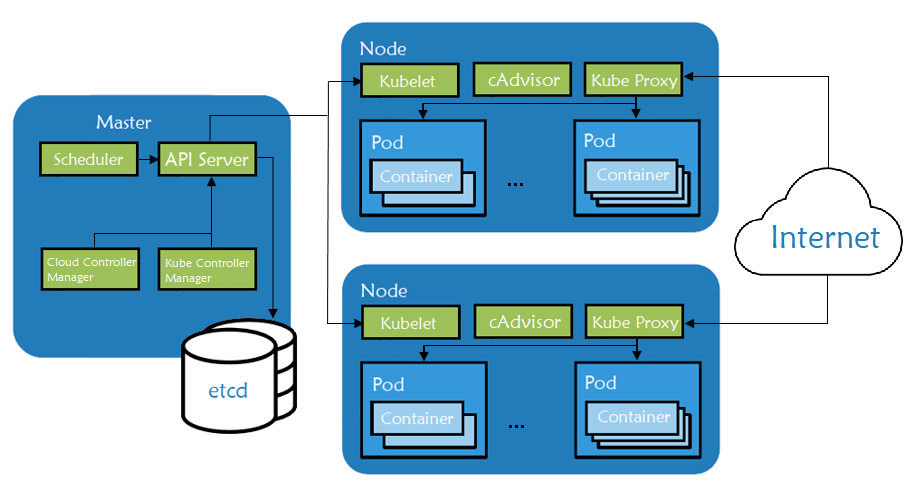
\includegraphics[scale=0.6]{figures/rancherK8sComponents.png}
    \caption{The Kubernetes Architecture and Node Components\cite{nodeSetupKubernetes:online}}
    \label{fig:nodeComponents}
\end{figure}
The kubelet is the primary node agent and schedules and maintains containers running inside a pod based on the pods \textit{PodSpecs}. It gets the these specifications mainly from the APIServer, but other Kubernetes internal sources are possible, too. Containers created outside of the cluster (or multi cluster) are not managed by the kubelet. 

Configuring the kubelet is easily possible via the kubectl and kubeadm tools which give the possibility of enhancing the kubelets performance for different circumstances, e.g. the edge. Going through the possible configurations under \url{https://kubernetes.io/docs/reference/command-line-tools-reference/kubelet/}, the most important configurations for the edge is the \textit{--housekeeping-interval duration} which defaults to 10s\cite{rancherKubernetesComponents:online}. This means each 10 seconds the kubelet performs a complete health check of all its components and sends it to the master. For normal cloud nodes this is a sensible choice. The nodes are powerful enough to handle the additional overhead and it avoids having unavailable resources. For light edge devices the interval is too high. The kubelet from k3s (discussed in \cref{sec:existingSolutions}) called hypervisor is compatible with vanilla Kubernetes and optimized for light edge devices.

For networking Kubernetes provides the kube-proxy which is a network proxy node agent ensuring that the Kubernetes networking services run on each node. It enables the Kubernetes service abstraction by ensuring the network rules on each host and carries out the connection forwarding. Kubernetes does not provide a standard implementation but requires the administrator to provide one at the installation. The last component, the container runtime (discussed in the \cref{sec:containers}), ensures that containers can run as expected.




% \vspace{0.5mm} \ \\
\textbf{\textit{Deployment Strategies}}\\
% \subsubsection{Deployment Strategies}
\comment{
deployment vs statefulset vs daemonset
clusterIP vs nodeport
Taints, nodeselector, affinities pod/node
namespaces
}
The \textit{service} resource provides an abstraction between the network interface and the actual application. From an outsiders view, it is possible to call the Kubernetes ingress gateway under a subsection and get to a pod running somewhere in the cluster without knowing its specific address. From the inside it enables routing between services based on the service name. Services are the usual deployment strategy for stateless applications. The pods are assigned a \textit{clusterIP} making it only accessible from inside the cluster, outside requests have to go through the cluster ingress and are then routed to a pod. This makes little sense on the edge, where latency is key and an Internet connection is not guaranteed. Instead, services offer the possiblity to define a \textit{nodePort} inside a service. It exposes a port from the pods to the host machine so that outside services can connect directly to the pod and the container listing for incoming connections.\\
Kubernetes also offers different resources for core workloads, \textit{Deployments},  \textit{StatefulSets},  \textit{DaemonSets} and  \textit{ReplicationController}, which should not be used anymore\cite{CoreWorkloadKubernetes66:online}. They all describe a desired state and the Kubernetes controller works towards fulfilling this desired state. Deployments are mainly used for stateless services. StatefulSets are used for stateful services and DaemonSets are to deploy pods on each node. For the edge all workloads are important, but it is important to choose the correct workload for a desired result. Inside the workloads specifications it is also possible to define resources. Because of the resource limitations of edge devices auto-scaling is not possible and devices can get quickly overwhelmed by too many tasks. This also puts an emphasis on the prioritization of workloads in case the hosts computing resources are not enough for all workloads.\\
Kubernetes offers powerful concepts to achieve the correct scheduling of pods on desired nodes. They are \textit{nodeSelector}, \textit{taints}, \textit{tollerations}, \textit{affinities} and \textit{anti-affinities}. A NodeSelector specifies which tags have to be present on a node for a pod to be scheduled on. Taints are added to nodes and specifies that only pods with the matching tolleration can run on the node. For exmaple, the master has the taint \textit{NoSchedule} which means, only pods with the matching tolleration can be scheduled on a the master. Finally, affinities and anti-affinities, offer a way for pods to be scheduled (or not) on either pods or nodes with a specific tag. This gives operators the ability to add workloads only on nodes which are already running another service, or with anit-affinity, where a pod is not present. Again, these are very powerful tools and have to be selected carefully.\\
Finally, \textit{namespaces} offer the ability to separate one physical cluster into mulitple virtual clusters. Most Kubernetes resources are saved inside namespaces which are especially important in a single-cluster setup with multiple user groups. Administrators can define namespaces and assign them resource limits as well as nodes via the \textit{PodNodeSelector}. This makes it possible to assign each logical edge deployment a virtual cluster and developers can only modify resources within that namespace. It is also possible to define role-based access control (RBAC) to limit what a specific user or user group can modify inside a namespace. 

\\[5mm]
\textbf{\leftskip25mm\textit{Load Balancing}}\\
Load balancing in a distributed environment is difficult as the ingress node needs a complete network topology at any given moment in time. This is one of the reasons why Kubernetes refreshes its node status so often. It also needs to synchronize this state across master nodes with a fast and distributed database called \textit{etcd}. External request go first to the master which needs to process and forward it to the right node. Load balancing is a perfect example why advantages and disadvantages of multi-cluster in contrast to single clusters have to be carefully weight. A full Kubernetes cluster on the edge comes with the advantage of having a full control plane on the edge and, thus, being able to load balance between nodes on the edge. 

But having a cluster at the edge comes with its downside. It needs a lot more management than a single cluster setup, consumes drastically more resources  and it needs a stable connection between the cluster nodes to work. But if resource consumption on the master is not an issue Kubernetes coupled with a load balancer provide more features and safeguarding than traditional (non orchestrated) load balancers do. Kubernetes always ensures that pods inside the cluster are healthy and reachable. If a pod goes down, Kubernetes will automatically schedule a new one. The internal load balancer can use this information and always route to an available pod. Other gateways like, Kong API Gateway or NGINX do not provide such features. Further, Kubernetes coupled with Istio makes it possible to do very fine grained traffic routing.

Finally, internal load balancing\footnote{Load balancing within one node.} is possible through normal API gateways and the deployment of multiple pods listening on different ports. For example, one NGINX container could function as load balancer for 5 containers on the same node. In Kubernetes this could be solved automatically with affinities. As soon as a node runs certain pods, a load balancer could automatically be side loaded.\\[5mm]
\textbf{\leftskip25mm\textit{Traffic Control and Shaping}}\\
% \subsubsection{Traffic Control and Shaping}
Traffic control and traffic shaping are very interesting edge topics. In Kubernetes each pod can be assigned incoming and outgoing bandwidth rates. But other tools extend this functionality and open up new possibilities. Istio, a service mesh mainly developed for Kubernetes, injects a sidecar proxy to fine tune the traffic of each container. It makes it possible to do rate limiting, control headers, reroute connection, change retries attempts, circuit breaking, mirroring and more while not changing the application code. Additionally, it is also able to encrypt traffic inside the mesh without the application knowing about it and gather all the telemetry data of the cluster. \\
With Kubernetes and tools extending its capabilities it is possible to do both traffic control and traffic shaping on a fine grained level. But, especially Istio, comes at the cost of additional overhead and the operator has to decide if the added functionality are worth the performance hit. Without Istio traffic control and shaping is only possible through the Kubernetes Ingress and thus in multi-cluster solutions.\\
Finally, Kubernetes is only meant to work with the Internet protocol stack and is only meant to operate within the clusters boundaries. So the actual communication with the IoT devices can not be controlled or shaped with Kubernetes.\\[0.5mm] 

\comment{
Removed section: Security and Recommendations
IIoT and the smartphone revolution have accelerated the need for fog computing and the industry is set to develop a container based orchestration tool, tightly integrated with Kubernetes. 
IIoT has accelerated the need for fog computing and the industry is set to develop a container based orchestration tool, tightly integrated with Kubernetes. The Kubernetes IoT edge working group was set up specifically to find the optimal Kubernetes strategy for the edge. However, it is not clear, whether the solution will be Kubernetes itslef or a more specialized tool. In this thesis I will argue that Kubernetes is the way forward as it already posses many of the features that are need for the edge.\\ 
}
\subsubsection{Containers} \label{sec:containers}
Containers first surfaced in 2007 with the release of Linux Containers (LXC). They provide an abstraction and isolation layer to the software they are supposed to run. Basically, a container is packaged software that runs independent from the underlying system. They are created at runtime from container images, which are packaged, standalone executable software including everything the main application needs to run (code, runtime, system tools, libraries and settings)\cite{containerDefinition:online}. Thus, containers offer
"unprecedented agility in developing and running applications in cloud environment especially when combined with a microservice-style architecture."\cite{microserviceContainers} Since 2007, there has been considered development of containers, especially by Docker, a company developing the same named application which is often used synonymously for containers. Docker donated its main container runtime environment, called containerd, to the CNCF open source community and later, in late 2017, announced the first major release of containerd. https://blog.docker.com/2017/12/cncf-containerd-1-0-ga-announcement/ This was significant, as the docker software was already widely used and it marked the start of an independent open source standard for containers.\\
Today, containers are the building blogs of the cloud and power almost all distributed applications. Craig McLuckie, the lead product manager cloud computing product at Google, said in a panel discussion during the Linux collaboration summit in Febraury 2015:
\begin{displayquote}
\textit{\textbf{\large{``}}}
\textit{This containers revolution is changing the basic act of software consumption. It’s redefining this much more lightweight, portable unit, or atom, that is much easier to manage... It’s a gateway to dynamic management and dynamic systems.}
\textit{\textbf{\large{''}}}
\end{displayquote}
It is important to note, that while the cloud saw the first transformation from containers the edge is part of the same dynamic system and stands to profit from adapting to containers. They offer many advantages over conventional deployments but have their drawbacks. For the edge resource consumption, hardware access and security are especially important and more closely analysed.\footnote{To keep the thesis concise I will not explain how containers work in greater detail only when required for the understanding of the content. For more information see Docker's website  \url{https://www.docker.com/resources/what-container} and containerd \url{https://containerd.io/}}.\\[0.5mm]

% \vspace{0.5mm} \ \\
\textbf{\textit{Resource Consumption}}\\
% \subsubsection{Resource consumption}
Processing power consumption from containers is always greater than bare metal deployments. However, recent research has shown that in most cases this is almost negligible. In an updated performance assessments of containers the authors found that containers introduce almost no overhead over a native deployment\cite{felter2015updatedPerformanceContainers}. By design containers share little with the default namespace, apart from system resources, like the kernel. It is possible to give containers access to host directories, but this often breaks their design philosophy of being stateless and portable. The solution is to include the libraries, tools, certificates necessary to run the application in the container itself. This can potentially lead to a ballooning size of containers and with multiple containers running simultaneously, disk space and memory consumption can easily exceed the system resources of an edge devices. E.g. deploying the latest official openJDK container consumes 470MB and only includes the runtime dependency for the JVM. Source and byte code and dependencies of the application would all add extra disk space on top of this. Compiled language are at a huge advantage in this regard. They compile to machine code and include all code dependencies in one binary. Some compiled languages even offer the possibility of cross-compilation. This means source code can be compiled for a different architecture they are being compiled on. This allows servers running on the x86 or amd64 architecture to compile to native ARM machine code.

Additionally, containers allow and encourage multi-stage builds. This method of building containers allows to have one container to build the application and another one to run the application. The one used for building contains all dependencies and the compile environment, while the one used for running the application only contains the binary and run-time relevant files (e.g. certificates or the linux user). This eliminates any unused files and is often used in combination with the \textit{scratch} image. 

It is the base image for all other images and is basically an empty file structure consuming no disk space or memory\footnote{It also creates an isolated network and process namespace, but they are also very cheap.}. According to Docker the scratch image ``is most useful in the context of building [...] super minimal images''\cite{scratchImageDockerD65:online}. Another advantage using smaller images is the faster extracting time. Images are usually stored as archives and extracted on the host machine placing an additional strain on the system for each new deployment.\\[0.5mm]
\comment{
Combining these these techniques can result in far lower memory and RAM consumption, but also better security (discussed in the next section). In the implementation, \cref{sec:testService} \nameref{sec:testService}, I will show just how much memory can be saved using these techniques. 




In an updated performance assessments of containers the authors found that containers introduce almost no overhead over a native deployment\cite{felter2015updatedPerformanceContainers}. Hence, gateways running Linux can in most cases use containers without a problem. 
}

% \vspace{0.5mm} \ \\
\textbf{\textit{Hardware Access}}\\
% \subsubsection{Hardware Access}
Hardware access is very important on the edge, but not so much in the cloud. Servers rarely communicate via different protocols or use different peripherals. On the edge access to bluetooth or usb sticks is very important. Sharing host resources with a container is possible through the \textit{privileged} flag set at deploy time. In a nutshell, a container has its own filesystem, network and process tree and cannot access resources outside of this scope. Using the \textit{privileged} flag gives a container access to the host containers resources. Containerd offers many ways to fine tune how much privileges the container should get. It is for example possible to only expose the hosts network namespace and not the process namespace or filesystem. 

\comment{
This is done in the implementation \cref{} \nameref{} to reduce security risks. However, these resources are not controlled by Kubernetes and need to be managed by the operator.


}

% \vspace{0.5mm} \ \\
\textbf{\textit{Security}}\\
% \subsubsection{Security}
Security is one of the biggest challenges in IoT. In 2016 a botnet with over 600k infected devices, primarily edge and IoT devices, overwhelmed several high-profile targets like the DNS provider Dyn with massive distributed denial-of-service (DDoS) attacks. This caused a temporary outage of their DNS servers rendering many webpages, among others  Twitter, Spotify and Amazon, temporally inaccessible. \\
In a recent talk at the Container Security Conference 2019 Andy Martin, co-founder of Control Plane, noted ``The root of all evil is unnecessarily running processes or containers as root''\cite{RootlessContainerSecurityTalk0:online}. This user can read, write and run all files in all directories. In the beginning of 2018 a new vulnerability on Kubernetes was discovered giving containers with volume mounts the ability to access data outside the volumes sub-path. The root user would thus have unlimited access to the host resources. To combat this, the user should be changed to a non-root and non-sudo enabled user. Running a container as privileged as in the previous section explained has further security implications and should only be used if necessary. It breaks down the isolation layers and allows the container to access and modify the hosts resources. Additionally, not providing a shell inside containers reduces the attack surface even further. It is also not possible to expose new ports from inside a container.\\
Using a compiled language adds further security. Binaries are resistant to code injection as well as other modifications and reverse engineering. Even if someone got a copy of the image, they could not detect how it works or alter it. Combined with the image digest they could not even sideload another application an repackage it as this would change the image digest. \\
Containers are usually downloaded from registries and most registries allow for overriding of image versions. If malicious attackers gain access to the registry they could potentially overwrite the latests version for a specific version tag. This would mean, all downloads by version tag would then download the malicious version. However, each image also has an image digest, a cryptographic signature ensuring that the image in question is the actual image. In production an image should always be pulled based on the image digest, also called "Pinning-by-Digest". So instead of unsing the download link \url{jonas27/hello:v1.0.1} the administrator should specify the image digest like so \url{jonas27/hello@sha256:725355347bc2eae8f7c9ab9dd09b9ef2c884b3458c693978f5408785aef1fb72}. This simple technique not only improves security but also guarantees that each container is derived from the same image. It also ensures that every instance of the service is running exactly the same code and combats race conditions.\\


\comment{
To combat malicious attacks certain methods have been developed. I will only analyze the direct container security aspects as they are always applicable for containers. Other methods, like specifically developed OSs and securing the CI/CD pipeline are not discussed at this point.\\

In the implementation \cref{sec:testService} \nameref{sec:testService} I will use the \textit{hello} service for testing. It's current version, v5arm, is saved on the Docker image hub and can be pulled with the link \textit{jonas27/hello:v5arm}. 

% \footnote{In this thesis I will only show deployments of containers with tags as they are referenced in multiple places for clarity. With Helm Charts this is profoundly easier but outside the scope of this thesis.} 


In conclusion, containers can significantly increase the isolation if some basics rules are followed. Use compiled language if possible, use the scratch image, do not include or expose more than needed and most importantly, don't use the root user if not absolutely necessary. When system resources are exposed it is even more important to properly secure the container. 
}



\comment{
https://www.iotforall.com/containers-on-the-edge/

 They isolate the application runtime and the 

Containers and Cloud: From LXC to Docker to Kubernetes

%  try use if vspace does not work \\[0.5mm]
}


\subsection{Standardization Efforts}
Standardization of technologies have huge implications on their usage. In a post from the IETF they say "standards form the fundamental building blocks for product development by establishing consistent protocols that can be universally understood and adopted". The Internet is build on open standards like HTTP, TCP, IP, HTML, URL and MAC which enabled it to thrive. It gives developers technical security and provides them an abstraction layer which they can develop against. Because of the novelty of running Kubernetes on the edge there is still considerable effort to standardize the edge components and communication protocols.\\[5mm]
% Standardization efforts IETF, CoAP (hadnled by IETF), CNCF edge working group, protobuf and grpc
{\textbf{\textit{Constrained Application Protocol}}}\\
Constrained Application Protocol (CoAP) is a "specialized web transfer protocol for use with constrained nodes and constrained networks"\cite{CoAPCon75:online} and is standardized under the IETF id 7252\cite{RFC7252CoAPIETF}. It is an application layer protocol similar to HTTP\textbackslash1 (or 2)  but utilizes UDP instead of TCP as transport layer protocol. The primary reason for this design choice is to keep the IP overhead as low as possible. It behaves similar to HTTP\textbackslash1 (or 2) in that it utilizes the REST model with a subset of its methods, e.g. \textit{GET, PUT, POST, DELETE} etc. Additionally, it offers caching of responses and proxying between CoAP and HTTP. It implements a stateful connection in the application layer rather than in transport layer and uses DTLS which works over unreliable data transfer connections. This is more efficient and does not require the typical three way handshake a TCP connection would require.

Compared to other IoT protocols CoAP is easier to understand as it uses the same concepts of the Internet stack. \Cref{fig:mqttVsCoap} shows side by side the architecture of Message Queuing Telemetry Transport (MQTT) and CoAP. Both are optimized for the IoT space and can do machine to machine (m2m), but their architecture is fundamentally different.
\begin{figure}[h!]
    \centering
    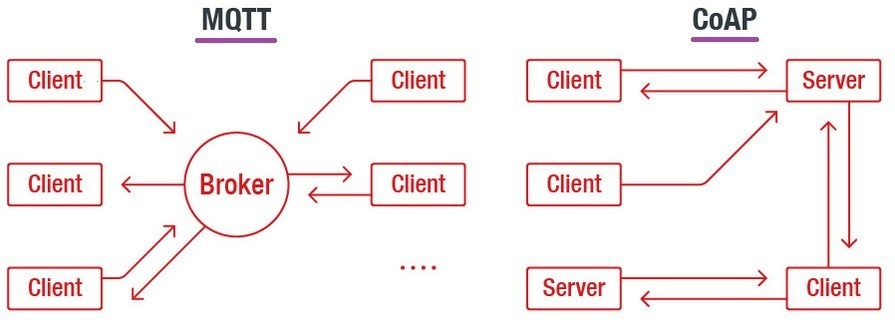
\includegraphics[scale=0.45]{figures/mqtt-vs-coap.jpg}
    \caption{MQTT and CoAP Architecture side by side\cite{COAPvsMQTT27:online}.}
    \label{fig:mqttVsCoap}
\end{figure}
MQTT is based on the publish-subscribe massaging pattern which relies on a central entity, called broker, to enable communication between multiple nodes. Researches compared the two standards and found "MQTT messages experienced lower delays than CoAP for lower packet loss and higher delays than CoAP for higher packet loss"\cite{MQTTvsCoAPAnalysisIEEE}. They also found that the message overhead for small messages is significantly lower at 25\% or less for CoAP compared to MQTT for reliable message transmission. But MQTT is by default synchronized across the cluster while CoAP is not. To combat this the standard was extended by the "observable" method in 2015\cite{RFC7641observableCoAP}. This makes it possible for a client to subscribe to a server resource and keep it updated by the server. and is very close to the publish-subscribe massaging pattern from MQTT.\\[5mm]
{\textbf{\textit{Protocol Buffers}}}\\
Protocol Buffers (Protobuf) are not yet standardized and only have an expired proposal under the IETF\cite{rfernando-protocol-buffers-00}. However, they are widely used for data serialization. Compared to JSON which is an IETF standard, protobufs are sent as binaries and thus not human readable. The protobuf message structure needs to be defined on the client and server side and represents an explicit contract of information exchange between the two. When an entity sends data as protobuf, the compiler appends an indicator of which field a binary string belongs to. Whereas in JSON both the identifier and the value are transmitted, in protobufs the identifier is a position in the data structure and put in front of its value.
When researches compared the message sizes of JSON to protobufs they found huge differences between the two, shown in \cref{fig:jsonVsProtobufs}.
\begin{figure}[H]
    \centering
    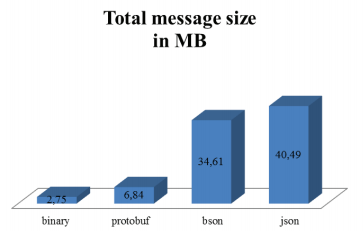
\includegraphics[scale=0.6]{figures/jsonVsProtobufs.png}
    \caption{Memory Consumption of different Serialization Protocols\cite{jsonVsProtobufs}.}
    \label{fig:jsonVsProtobufs}
\end{figure}
The researches conclude "the Protocol Buffers are a serious candidate for standardized way of communication in field of Internet of Things"\cite{jsonVsProtobufs}.\\[5mm]
{{\textbf{\textit{Kubernetes IoT Edge working group}}}}\\
The Kubernetes IoT Edge working group\cite{IntroducingDejanBosanac:KubernetesIoTEdgeWorkingGroup} was introduced in mid 2018 and is a platform for companies to develop open edge standards in connection with Kubernetes. The Cloud Native Computing Foundry (CNCF) under which Kubernetes resides "saw more and more developers trying to use Kubernetes outside typical data center deployments"\cite{IntroducingDejanBosanac:KubernetesIoTEdgeWorkingGroup}, especially on the edge. It wants to bring the cloud-native best practices and tools to the edge. The projects proposed in the working group are not all based on Kubernetes but are supposed to seamlessly integrate into its existing workflow. The group has identified many problem areas Kubernetes is not yet ready to deal with. This includes trusting of unconnected hardware, trusting of connected devices, secure operating system, network concerns and integrity of software. These areas are immensely important and an open solution would have a huge impact on the edge industry, just as Kubernetes had for the cloud industry.





\comment{
Should I include Azure IoT Edge as managed cloud iot gateway offering????\\

The problems at the IoT edge, connectivity, manageability, scalability, reliability, security, are being solved as point solutions by enterprises and ecosystem players, there is a need for a foundational industry-wide standard for managing distributed IoT workloads.


What is the purpose of this section?\\
problem area: what is actually the problem with the current system? hint into solution\\
competitor anaylsis: compare different approaches to solve the management and security of IoT gateways as well as solutions inside the individual categories. 


}